% Project architecture diagram. Build: pdflatex project-architecture.tex
\documentclass{article}
\usepackage[paperwidth=34cm,paperheight=21.5cm,margin=0.6cm]{geometry}
\usepackage{tikz}
\usetikzlibrary{arrows.meta,positioning,fit,backgrounds,calc}
\usepackage[T1]{fontenc}
\usepackage{lmodern}
\pagestyle{empty}

\definecolor{cin}{HTML}{3f6fb5}    % inputs
\definecolor{cfound}{HTML}{3a7d6b} % shared foundations
\definecolor{chyp}{HTML}{c2662d}   % ideas -> hypotheses
\definecolor{cout}{HTML}{6b6b6b}   % outputs
\definecolor{cgov}{HTML}{8c7a5a}   % governance

\tikzset{
  box/.style={draw=#1, fill=#1!8, rounded corners=3pt, line width=0.7pt, align=left,
              inner sep=5pt, font=\footnotesize, anchor=north west},
  plan/.style={box=#1, dashed, fill=white},
  ttl/.style={font=\bfseries\small},
  col/.style={font=\bfseries\large, text=#1, anchor=south west},
  arr/.style={-{Stealth[length=2.6mm]}, line width=0.8pt, draw=black!60},
  lab/.style={font=\scriptsize\itshape, text=black!70, fill=white, inner sep=1.5pt},
}
\newcommand{\pth}[1]{\texttt{#1}}

\begin{document}
\noindent
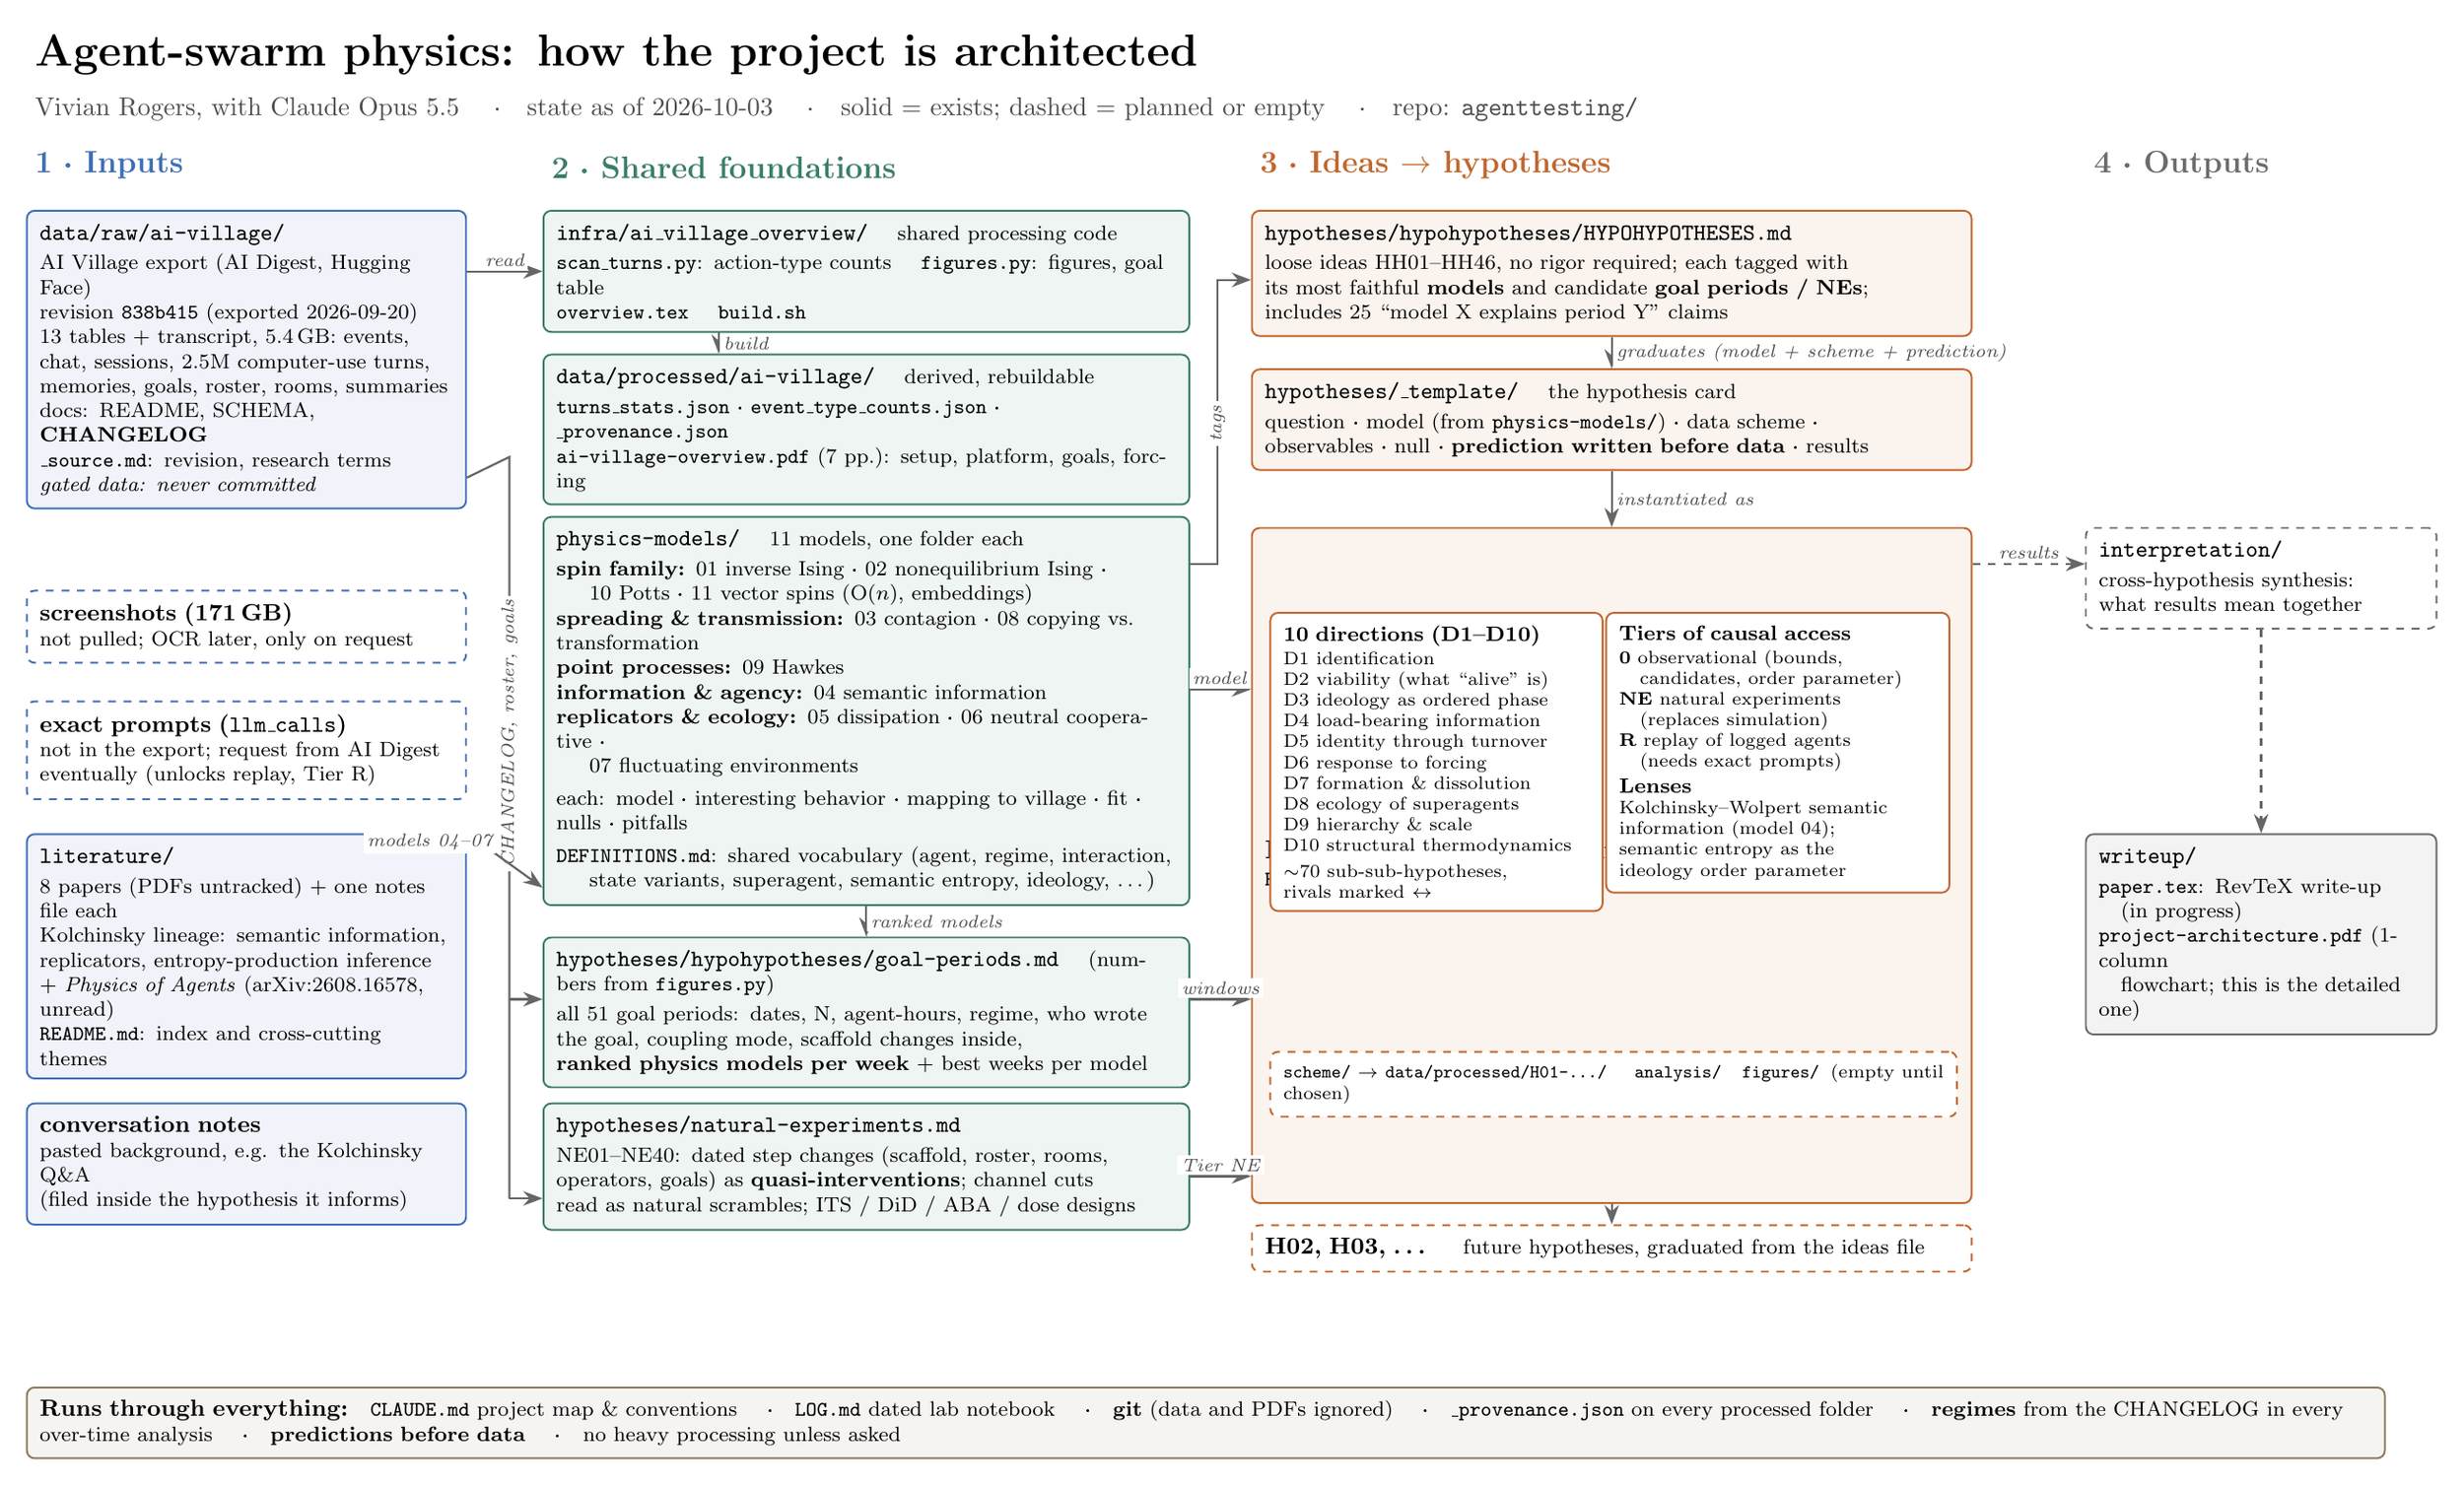
\begin{tikzpicture}[x=1cm,y=1cm]

% ---------------- title
\node[anchor=north west, font=\bfseries\LARGE] at (0,20.2) {Agent-swarm physics: how the project is architected};
\node[anchor=north west, font=\normalsize, text=black!70] at (0,19.35)
  {Vivian Rogers, with Claude Opus 5.5 \quad·\quad state as of 2026-10-03 \quad·\quad solid = exists; dashed = planned or empty \quad·\quad repo: \pth{agenttesting/}};

% ---------------- column headers
\node[col=cin]    at (0,18.0)   {1 · Inputs};
\node[col=cfound] at (7.0,18.0) {2 · Shared foundations};
\node[col=chyp]   at (16.6,18.0){3 · Ideas $\rightarrow$ hypotheses};
\node[col=cout]   at (27.9,18.0){4 · Outputs};

% ================= 1. INPUTS
\node[box=cin, text width=5.6cm] (raw) at (0,17.7) {%
  {\bfseries\small \pth{data/raw/ai-village/}}\\[2pt]
  AI Village export (AI Digest, Hugging Face)\\
  revision \pth{838b415} (exported 2026-09-20)\\
  13 tables + transcript, 5.4\,GB: events,\\
  chat, sessions, 2.5M computer-use turns,\\
  memories, goals, roster, rooms, summaries\\
  docs: README, SCHEMA, \textbf{CHANGELOG}\\
  \pth{\_source.md}: revision, research terms\\
  \emph{gated data: never committed}};

\node[plan=cin, text width=5.6cm] (shots) at (0,12.55) {%
  {\bfseries\small screenshots (171\,GB)}\\
  not pulled; OCR later, only on request};

\node[plan=cin, text width=5.6cm] (prompts) at (0,11.05) {%
  {\bfseries\small exact prompts (\pth{llm\_calls})}\\
  not in the export; request from AI Digest\\
  eventually (unlocks replay, Tier R)};

\node[box=cin, text width=5.6cm] (lit) at (0,9.25) {%
  {\bfseries\small \pth{literature/}}\\[2pt]
  8 papers (PDFs untracked) + one notes file each\\
  Kolchinsky lineage: semantic information,\\
  replicators, entropy-production inference\\
  + \emph{Physics of Agents} (arXiv:2608.16578, unread)\\
  \pth{README.md}: index and cross-cutting themes};

\node[box=cin, text width=5.6cm] (conv) at (0,5.6) {%
  {\bfseries\small conversation notes}\\
  pasted background, e.g. the Kolchinsky Q\&A\\
  (filed inside the hypothesis it informs)};

% ================= 2. SHARED FOUNDATIONS
\node[box=cfound, text width=8.4cm] (infra) at (7.0,17.7) {%
  {\bfseries\small \pth{infra/ai\_village\_overview/}} \quad shared processing code\\[2pt]
  \pth{scan\_turns.py}: action-type counts \quad \pth{figures.py}: figures, goal table\\
  \pth{overview.tex} \quad \pth{build.sh}};

\node[box=cfound, text width=8.4cm] (proc) at (7.0,15.75) {%
  {\bfseries\small \pth{data/processed/ai-village/}} \quad derived, rebuildable\\[2pt]
  \pth{turns\_stats.json} · \pth{event\_type\_counts.json} · \pth{\_provenance.json}\\
  \textbf{\pth{ai-village-overview.pdf}} (7 pp.): setup, platform, goals, forcing};

\node[box=cfound, text width=8.4cm] (pm) at (7.0,13.55) {%
  {\bfseries\small \pth{physics-models/}} \quad 11 models, one folder each\\[2pt]
  \textbf{spin family:} 01 inverse Ising · 02 nonequilibrium Ising ·\\
  \hspace*{1.5em}10 Potts · 11 vector spins (O($n$), embeddings)\\
  \textbf{spreading \& transmission:} 03 contagion · 08 copying vs.\ transformation\\
  \textbf{point processes:} 09 Hawkes\\
  \textbf{information \& agency:} 04 semantic information\\
  \textbf{replicators \& ecology:} 05 dissipation · 06 neutral cooperative ·\\
  \hspace*{1.5em}07 fluctuating environments\\[3pt]
  each: model · interesting behavior · mapping to village · fit · nulls · pitfalls\\[3pt]
  \textbf{\pth{DEFINITIONS.md}}: shared vocabulary (agent, regime, interaction,\\
  \hspace*{1.5em}state variants, superagent, semantic entropy, ideology, …)};

\node[box=cfound, text width=8.4cm] (gp) at (7.0,7.85) {%
  {\bfseries\small \pth{hypotheses/hypohypotheses/goal-periods.md}} \quad (numbers from \pth{figures.py})\\[2pt]
  all 51 goal periods: dates, N, agent-hours, regime, who wrote\\
  the goal, coupling mode, scaffold changes inside,\\
  \textbf{ranked physics models per week} + best weeks per model};

\node[box=cfound, text width=8.4cm] (ne) at (7.0,5.6) {%
  {\bfseries\small \pth{hypotheses/natural-experiments.md}}\\[2pt]
  NE01–NE40: dated step changes (scaffold, roster, rooms,\\
  operators, goals) as \textbf{quasi-interventions}; channel cuts\\
  read as natural scrambles; ITS / DiD / ABA / dose designs};

% ================= 3. IDEAS -> HYPOTHESES
\node[box=chyp, text width=9.4cm] (hh) at (16.6,17.7) {%
  {\bfseries\small \pth{hypotheses/hypohypotheses/HYPOHYPOTHESES.md}}\\[2pt]
  loose ideas HH01–HH46, no rigor required; each tagged with\\
  its most faithful \textbf{models} and candidate \textbf{goal periods / NEs};\\
  includes 25 ``model X explains period Y'' claims};

\node[box=chyp, text width=9.4cm] (tmpl) at (16.6,15.55) {%
  {\bfseries\small \pth{hypotheses/\_template/}} \quad the hypothesis card\\[2pt]
  question · model (from \pth{physics-models/}) · data scheme ·\\
  observables · null · \textbf{prediction written before data} · results};

\node[box=chyp, text width=9.4cm, minimum height=9.15cm] (h01) at (16.6,13.4) {%
  {\bfseries\normalsize H01 · Emergent superagents exist} \quad (status: idea)\\[1pt]
  \pth{README.md} card · \pth{architecture.md} · \pth{subhypotheses.md} · \pth{notes/}};

% inner content of H01
\node[box=chyp, fill=white, text width=4.15cm, font=\scriptsize] (dirs) at (16.85,12.25) {%
  {\bfseries\footnotesize 10 directions (D1–D10)}\\[1pt]
  D1 identification\\
  D2 viability (what ``alive'' is)\\
  D3 ideology as ordered phase\\
  D4 load-bearing information\\
  D5 identity through turnover\\
  D6 response to forcing\\
  D7 formation \& dissolution\\
  D8 ecology of superagents\\
  D9 hierarchy \& scale\\
  D10 structural thermodynamics\\[2pt]
  $\sim$70 sub-sub-hypotheses,\\ rivals marked $\leftrightarrow$};

\node[box=chyp, fill=white, text width=4.3cm, font=\scriptsize] (tiers) at (21.4,12.25) {%
  {\bfseries\footnotesize Tiers of causal access}\\[1pt]
  \textbf{0} observational (bounds,\\ \hspace*{1em}candidates, order parameter)\\
  \textbf{NE} natural experiments\\ \hspace*{1em}(replaces simulation)\\
  \textbf{R} replay of logged agents\\ \hspace*{1em}(needs exact prompts)\\[2pt]
  {\bfseries\footnotesize Lenses}\\
  Kolchinsky--Wolpert semantic\\ information (model 04);\\
  semantic entropy as the\\ ideology order parameter};

\node[plan=chyp, text width=8.95cm, font=\scriptsize] (h01s) at (16.85,6.3) {%
  \pth{scheme/} $\rightarrow$ \pth{data/processed/H01-…/} \quad\pth{analysis/}\quad\pth{figures/} \hfill (empty until chosen)};

\node[plan=chyp, text width=9.4cm] (hnext) at (16.6,3.95) {%
  {\bfseries\small H02, H03, …} \quad future hypotheses, graduated from the ideas file};

% ================= 4. OUTPUTS
\node[plan=cout, text width=4.4cm] (interp) at (27.9,13.4) {%
  {\bfseries\small \pth{interpretation/}}\\[2pt]
  cross-hypothesis synthesis:\\ what results mean together};

\node[box=cout, text width=4.4cm] (wu) at (27.9,9.25) {%
  {\bfseries\small \pth{writeup/}}\\[2pt]
  \pth{paper.tex}: RevTeX write-up\\ \hspace*{1em}(in progress)\\
  \pth{project-architecture.pdf} (1-column\\ \hspace*{1em}flowchart; this is the detailed one)};

% ================= governance band
\node[box=cgov, text width=31.6cm, font=\footnotesize] (gov) at (0,1.75) {%
  {\bfseries\small Runs through everything:}\quad
  \textbf{\pth{CLAUDE.md}} project map \& conventions \quad·\quad
  \textbf{\pth{LOG.md}} dated lab notebook \quad·\quad
  \textbf{git} (data and PDFs ignored) \quad·\quad
  \textbf{\pth{\_provenance.json}} on every processed folder \quad·\quad
  \textbf{regimes} from the CHANGELOG in every over-time analysis \quad·\quad
  \textbf{predictions before data} \quad·\quad
  no heavy processing unless asked};

% ================= arrows (routed through the gaps between columns)
% raw -> infra
\draw[arr] (raw.east |- infra.west) -- node[lab, above]{read} (infra.west);
% raw -> goal periods and natural experiments, via a bus at x = 6.55
\draw[line width=0.8pt, draw=black!60] ($(raw.east)+(0,-1.6)$) -- (6.55,{15.95-1.6}) -- (6.55,4.3);
\draw[arr] (6.55,7.0) -- (gp.west |- 0,7.0);
\draw[arr] (6.55,4.3) -- (ne.west |- 0,4.3);
\node[lab, rotate=90] at (6.55,10.6) {CHANGELOG, roster, goals};
% infra -> processed
\draw[arr] ($(infra.south)+(-2,0)$) -- node[lab, right]{build} ($(proc.north)+(-2,0)$);
% literature -> models
\draw[arr] (lit.north east) -- node[lab, above left, pos=0.4]{models 04--07} ($(pm.south west)+(0,0.25)$);
% models -> goal periods
\draw[arr] (pm.south) -- node[lab, right]{ranked models} (gp.north);
% models -> ideas (tags), via x = 16.15
\draw[arr] (15.75,12.9) -- (16.15,12.9) -- (16.15,16.75) -- (hh.west |- 0,16.75);
\node[lab, rotate=90] at (16.15,14.8) {tags};
% models -> H01
\draw[arr] (15.75,11.2) -- node[lab, above]{model} (h01.west |- 0,11.2);
% goal periods -> H01, NEs -> H01
\draw[arr] (gp.east |- 0,7.0) -- node[lab, above]{windows} (h01.west |- 0,7.0);
\draw[arr] (ne.east |- 0,4.6) -- node[lab, above]{Tier NE} (h01.west |- 0,4.6);
% ideas -> template -> H01 -> next
\draw[arr] (hh.south) -- node[lab, right]{graduates (model + scheme + prediction)} (tmpl.north);
\draw[arr] (tmpl.south) -- node[lab, right]{instantiated as} (h01.north);
\draw[arr, dashed] (h01.south) -- (hnext.north);
% H01 -> interpretation -> writeup
\draw[arr, dashed] (h01.east |- 0,12.9) -- node[lab, above]{results} (interp.west |- 0,12.9);
\draw[arr, dashed] (interp.south) -- (wu.north);

\end{tikzpicture}
\end{document}
